\documentclass[12pt]{article}
\usepackage{graphicx}
\usepackage{pdfpages}
\graphicspath{ {./figures/} }
\title{Timeline to Final Review}
\author{Mostafa Rizk}

\begin{document}

\maketitle

Following the recommendations of the panel, and in discussion with my supervisors, I have streamlined my research to focus on 3 research questions. The timeline below (Section \ref{timeline}) consists of 4 groups of tasks, one for each research question and one for the literature review, which is ongoing parallel to the other 3 groups. 
The timeline goes from the last 2 work weeks of 2020 through to the reconvene seminar in April. 
Work after the seminar will be primarily thesis writeup. 
Sections \ref{group_1}, \ref{group_2}, \ref{group_3} and \ref{group_4} explain each group of tasks.
Section \ref{learning} in the appendix contains a clarification of the learning process to aid in understanding some of the tasks.

\section{Group 1- Landscape Analysis}\label{group_1}

For this group of tasks, I perform RWG analysis, as described in \cite{oller:AAMAS:2020}  to understand the fitness landscape for the centralised setup. 
This involves randomly sampling a team of agents (specifically 2 agents) several thousand times, evaluating the team and visualising the distribution of team scores. 
I can then make inferences about things like the gradient of the landscape and the presence of local optima.

\subsection{Creating a Fitness Gradient}

One possible shortcoming of this part of the research is that the fitness function might be making the problem unnecessarily difficult.\\

\textbf{Hypothesis 1.1:} Rewarding agents for partial retrieval of the resource will create a smoother fitness gradient that evolution could then take advantage of.\\

Investigating this hypothesis is the first task in the group.
I conducted an experiment to test this hypothesis where I repeated the landscape analysis but with incremental rewards.
The results of this experiment are in Section \ref{smooth_fitness} of the appendix.

\subsection{Visualising Specialisation}\label{visualising_specialisation}

I already performed the initial analysis of the landscape, however, the visualisation did not contain any information about how specialised each team was i.e. was a given solution a pair of generalists or a pair of specialists? 
Are the better solutions in the landscape usually specialists? 
How common are specialist solutions compared to generalist ones? 
To visualise this information I need a way of measuring the degree of specialisation of a solution, so the second task in this group is to evaluate some candidate metrics and the third is to incorporate the chosen metric into the landscape analysis.\\

\textbf{Hypothesis 1.2:} The fittest solutions in the landscape are the specialised ones but they are also rarer than generalist solutions.\\

\subsection{Dimensionality Reduction}

I have also included dimensionality reduction as part of the third task.
Following the seminar, I discovered a technique to project the fitness landscape in two dimensions, which lets me visualise how far apart solutions are.
This technique, Sammon's mapping \cite{sammon:IEEETR:1969}, has been used in other work \cite{kim:GECCO:2003, risi:AB:2010} to visualise landscapes for agent-based problems.
Combined with the specialisation metric, this answers additional questions that are also significant.
How far apart are specialist and generalist solutions in the landscape?
How many optima are there?
What trajectory does evolution take through the landscape?
I have already implemented this technique and started to get preliminary answers.\\

\textbf{Hypothesis 1.3:} There are two optima in the landscape, a specialist one and a generalist one, and the specialist optima has fitter solutions. \\

\subsection{Analysis of Different Slope Angles}

The fourth task is to redo the analysis using different slope angles. 
This means randomly sampling teams of agents as before, but evaluating them in environments where the slope is different. 
Changing the slope angle changes how beneficial specialisation is. 
Having no slope at all means there should be no benefit from specialisation and no pressure for agents to learn it.\\

\textbf{Hypothesis 1.4:} When the slope is flat, no solutions in the landscape will be specialists and when the slope is steep, the specialised solutions will be higher-scoring.\\

\subsection{Optional Tasks}

The two optional tasks are to get a more thorough understanding of the landscape, if time allows, by considering the landscape for the decentralised setup and for a more complex version of the environment.\\

\subsubsection{Decentralised Setup Analysis} 

The current landscape analysis shows the landscape for a centralised algorithm because it plots solutions for the team as a whole. 
For the decentralised algorithm, the fitness landscape is not static because an agent’s fitness depends on who it is paired with. 
The features of the landscape, therefore, are likely to be different for the decentralised approach. 
This task involves modifying the current landscape analysis to give insight into the landscape for the decentralised setup.
One way of doing this is by using the dimensionality reduction technique from Section \ref{visualising_specialisation}.
Consider 2-agent teams in the centralised setup.
A solution in the landscape is the genomes of both agents on the team.
Consider now a 2-agent team in the decentralised setup.
Each agent has its own fitness landscape, but if we take both agents on the team and concatenate their genomes, we can plot that team in the same landscape as the centralised teams.
This does not tell us what the landscape is like for each agent during the learning process, but it shows us how the decentralised algorithm navigates the shared fitness landscape compared to the centralised algorithm.
Does the decentralised algorithm ultimately find the same solutions as the centralised one?\\

\textbf{Hypothesis 1.5:} Solutions found by the decentralised algorithm will be primarily generalist whereas solutions found by the centralised algorithm will be primarily specialist.\\

\subsubsection{Analysing Complex Environments}
The current task is relatively simple. 
How does the landscape change when the task becomes more challenging?

\section{Group 2- Centralised vs Decentralised}\label{group_2}

Following from the description of the learning process in Appendix Section \ref{learning} :\\

\textbf{Hypothesis 2.1:} Centralised learning finds specialisation more frequently. \\

Since centralised learning is trying to find the best team solution and specialisation is what is best for the team, it should more frequently find specialisation than decentralised learning. 
In decentralised learning, each agent’s learning process is trying to find the best solution in an environment where it does not know who it will be partnered with. 
The best solution should thus be the safest one, which is a generalist behaviour.\\

\textbf{Hypothesis 2.2:} Decentralised learning scales better than centralised learning. \\

For centralised learning, since it is searching for a team solution, the search space grows rapidly as the number of agents increases, so we can expect learning to find worse solutions for larger teams. 
These solutions should be less fit but it is not clear if they will also be less specialised.\\

For decentralised learning, the space of solutions remains the same for each agent, when the team size increases, however, there are more concurrent learning processes. 
An agent’s score depends on many other agents executing unknown strategies in its environment, and all those strategies affect one another, so the increased noise may also make it difficult to find good solutions for larger teams.\\

\textbf{Hypothesis 2.3:} Decentralised learning is more robust to changes in the team (as measured by the fitness of solutions).\\

As stated in Hypothesis 2.1, decentralised learning should find the safest strategy for an agent, i.e. a generalist strategy. This strategy is successful regardless of the strategies of its teammates. If an agent is evaluated with new teammates it has never been paired with before, it should still perform reasonably well. \\

Conversely, an agent from the centralised setup is part of a larger solution. It is likely specialised. We can expect that if the agent is paired with new teammates, the team performance will suffer. \\

The first task in this group is to do some code fixes to facilitate the experiments that will answer the hypotheses.
The second task answers Hypothesis 2.2 and the third answers Hypothesis 2.3, while both together answer Hypothesis 2.1 as specialisation can be measured for the solutions in both.


\section{Group 3- Price of Anarchy}\label{group_3}

Theoretically, centralised learning is equivalent to a benevolent dictator that assigns roles to each agent on the team so that the collective solution is socially optimal. 
Decentralised learning is equivalent to a group of self-interested individuals where each is trying to find what is best for itself and we expect that is less likely to find a socially optimal solution. 
Calculating the price of anarchy lets us determine how far the team performance drops when agents are self-interested, i.e. how much performance should drop when using decentralised as opposed to centralised learning.\\

\textbf{Hypothesis 3.1:} The slope foraging problem is a stag hunt with two Nash equilibria, where the payoff-dominant equilibrium is specialist solutions and the risk-dominant is generalist solutions.\\

\textbf{Hypothesis 3.2:} The centralised setup is more likely to find the payoff-dominant Nash equilibrum while the decentralised setup is more likely to find the risk-dominant Nash equilibrium.\\

\section{Group 4- Literature Review}\label{group_4}

I have created a spreadsheet to systematically keep track of the literature and ensure my research is supported by a firm knowledge of the field. 
Throughout the next few months, I will add relevant papers to the spreadsheet as I delve deeper into each research question, doing brief first passes of each to get an overview and deeper second and third passes for any that are especially relevant.

\section{Timeline} \label{timeline}

\includepdf{refined_timeline.pdf}

\bibliographystyle{ieeetr}
\bibliography{references}

\appendix

\section{The Learning Process}\label{learning}

Each agent is controlled by its own neural network. 
The network encodes the agent’s behaviour i.e. it encodes a function that maps from local observations to actions. 
The neural network architecture is fixed, but the weights are changed throughout the learning process.\\

\subsection{Centralised}

In the centralised setup, a learning algorithm creates a population of solutions. 
A solution is a sequence of neural network weights for the network of each agent on the team. 
For example, if a network has 50 weights and there are 4 agents, the solution has a length of 200. 
Each part of the solution is assigned to a random agent. 
The agents then carry out several episodes, starting from random positions at the nest each episode and acting for a fixed number of time steps. 
The score is calculated at the end of each episode and it is the sum of rewards for all resources gathered by the team minus the costs paid by all agents. 
The average score over all episodes is calculated and used to create a new population of solutions. 
This repeats until the algorithm terminates.\\

\subsection{Decentralised}

The decentralised setup has changed since the seminar and now uses a technique called cooperative coevolution. 
In cooperative coevolution, rather than one evolutionary process learning a combined solution for the entire team, each agent on the team has its own evolutionary process learning a solution for only itself. 
For example, if there are 4 agents, there are 4 evolutionary processes running concurrently. 
At generation $i$, each of the 4 processes creates a population of solutions for its agent, where a solution is the weights of a single agent’s neural network. 
The score of a solution at generation i is calculated by pairing it with the best solutions from each of the other 3 agents’ evolutionary processes at generation $i-1$. 
The score is for that single agent’s performance; it is the team reward (total resources collected) divided by the number of agents (regardless of their contribution) minus the cost incurred by that particular agent.\\

\subsection{Difference}

The difference between centralised and decentralised is that a centralised algorithm uses one learning process to learn a solution for the entire team whereas the decentralised algorithm uses multiple concurrent learning processes to learn solutions for each agent independently that are then combined. 
Centralised learning rewards the team while decentralised learning rewards the individual.\\

\section{Creating a Fitness Gradient}\label{smooth_fitness}

\textbf{Hypothesis 1.1:} Rewarding agents for partial retrieval of the resource will create a smoother fitness gradient that evolution could then take advantage of.\\

I divided the reward for retrieving a resource by the length of the arena and gave agents part of the reward if they moved the resource a single tile closer to the goal.
The plots for the original landscape analysis and the analysis with the new fitness function are shown in Figure \ref{fig:sparse} and Figure \ref{fig:incremental} respectively.\\

\begin{figure}[h]
\centering
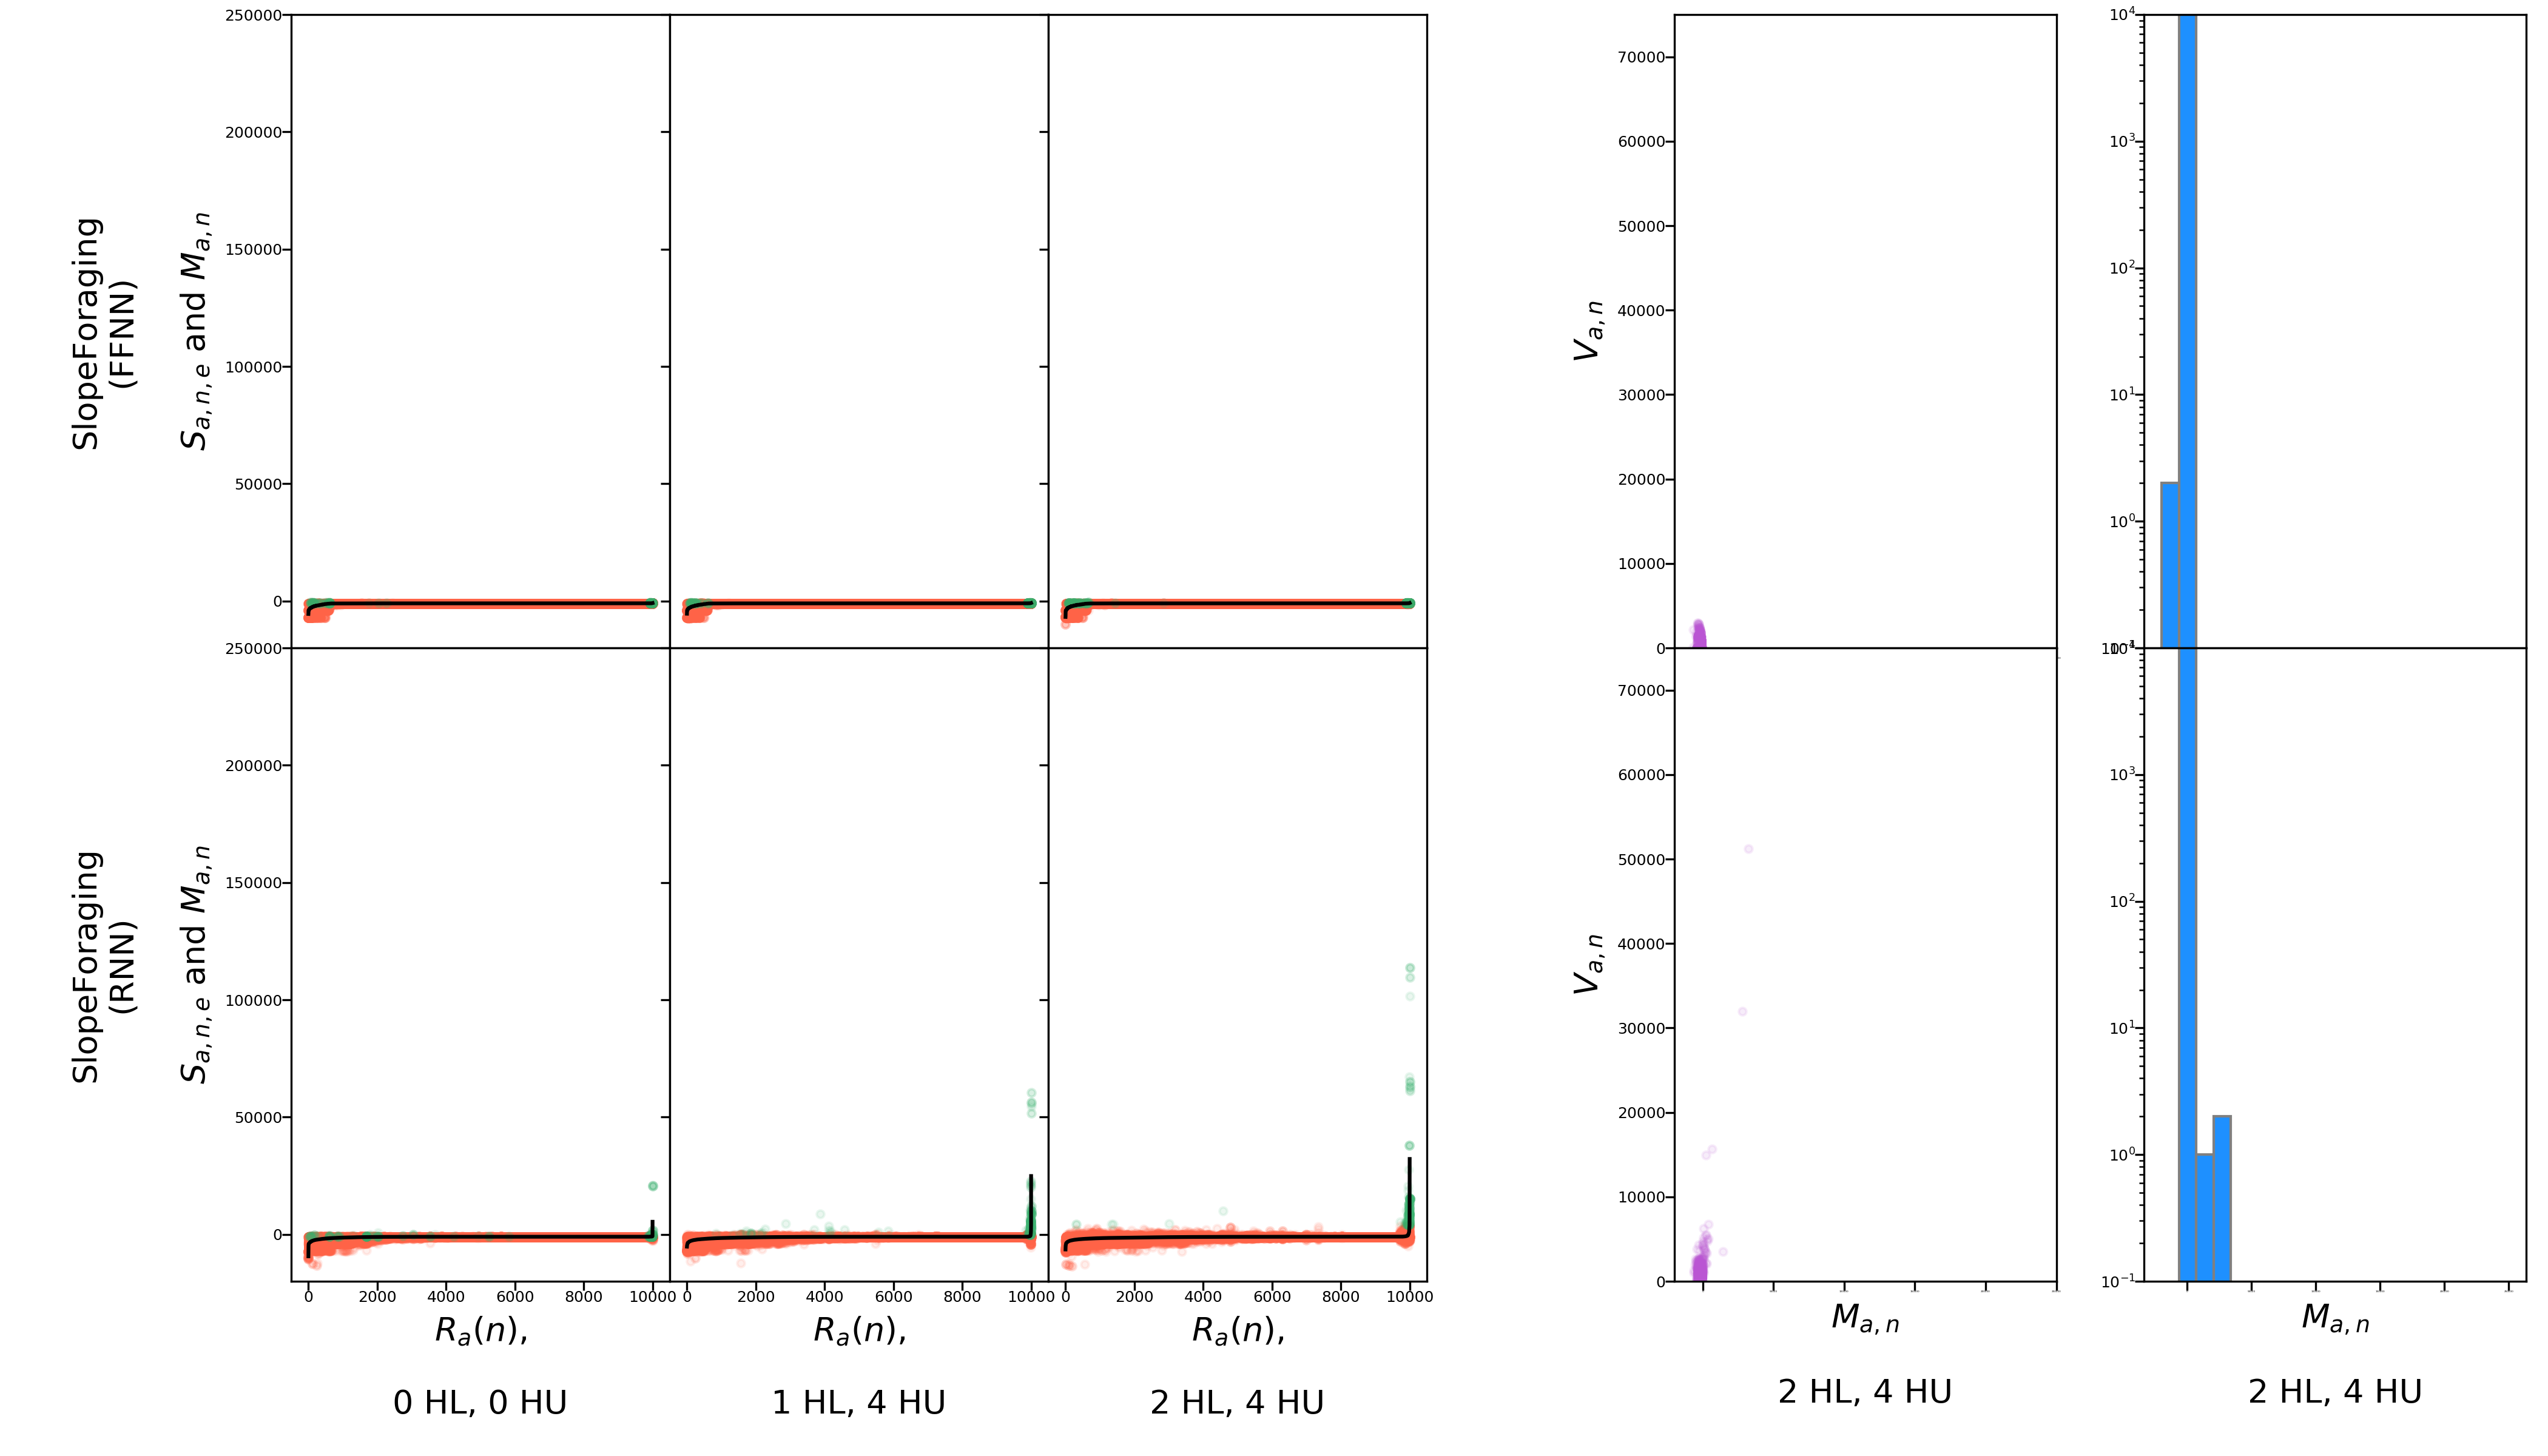
\includegraphics[width=1.0\textwidth]{sparse_rewards.png}
\caption{RWG Analysis with the original fitness function}
\label{fig:sparse}
\end{figure}

\begin{figure}[h]
\centering
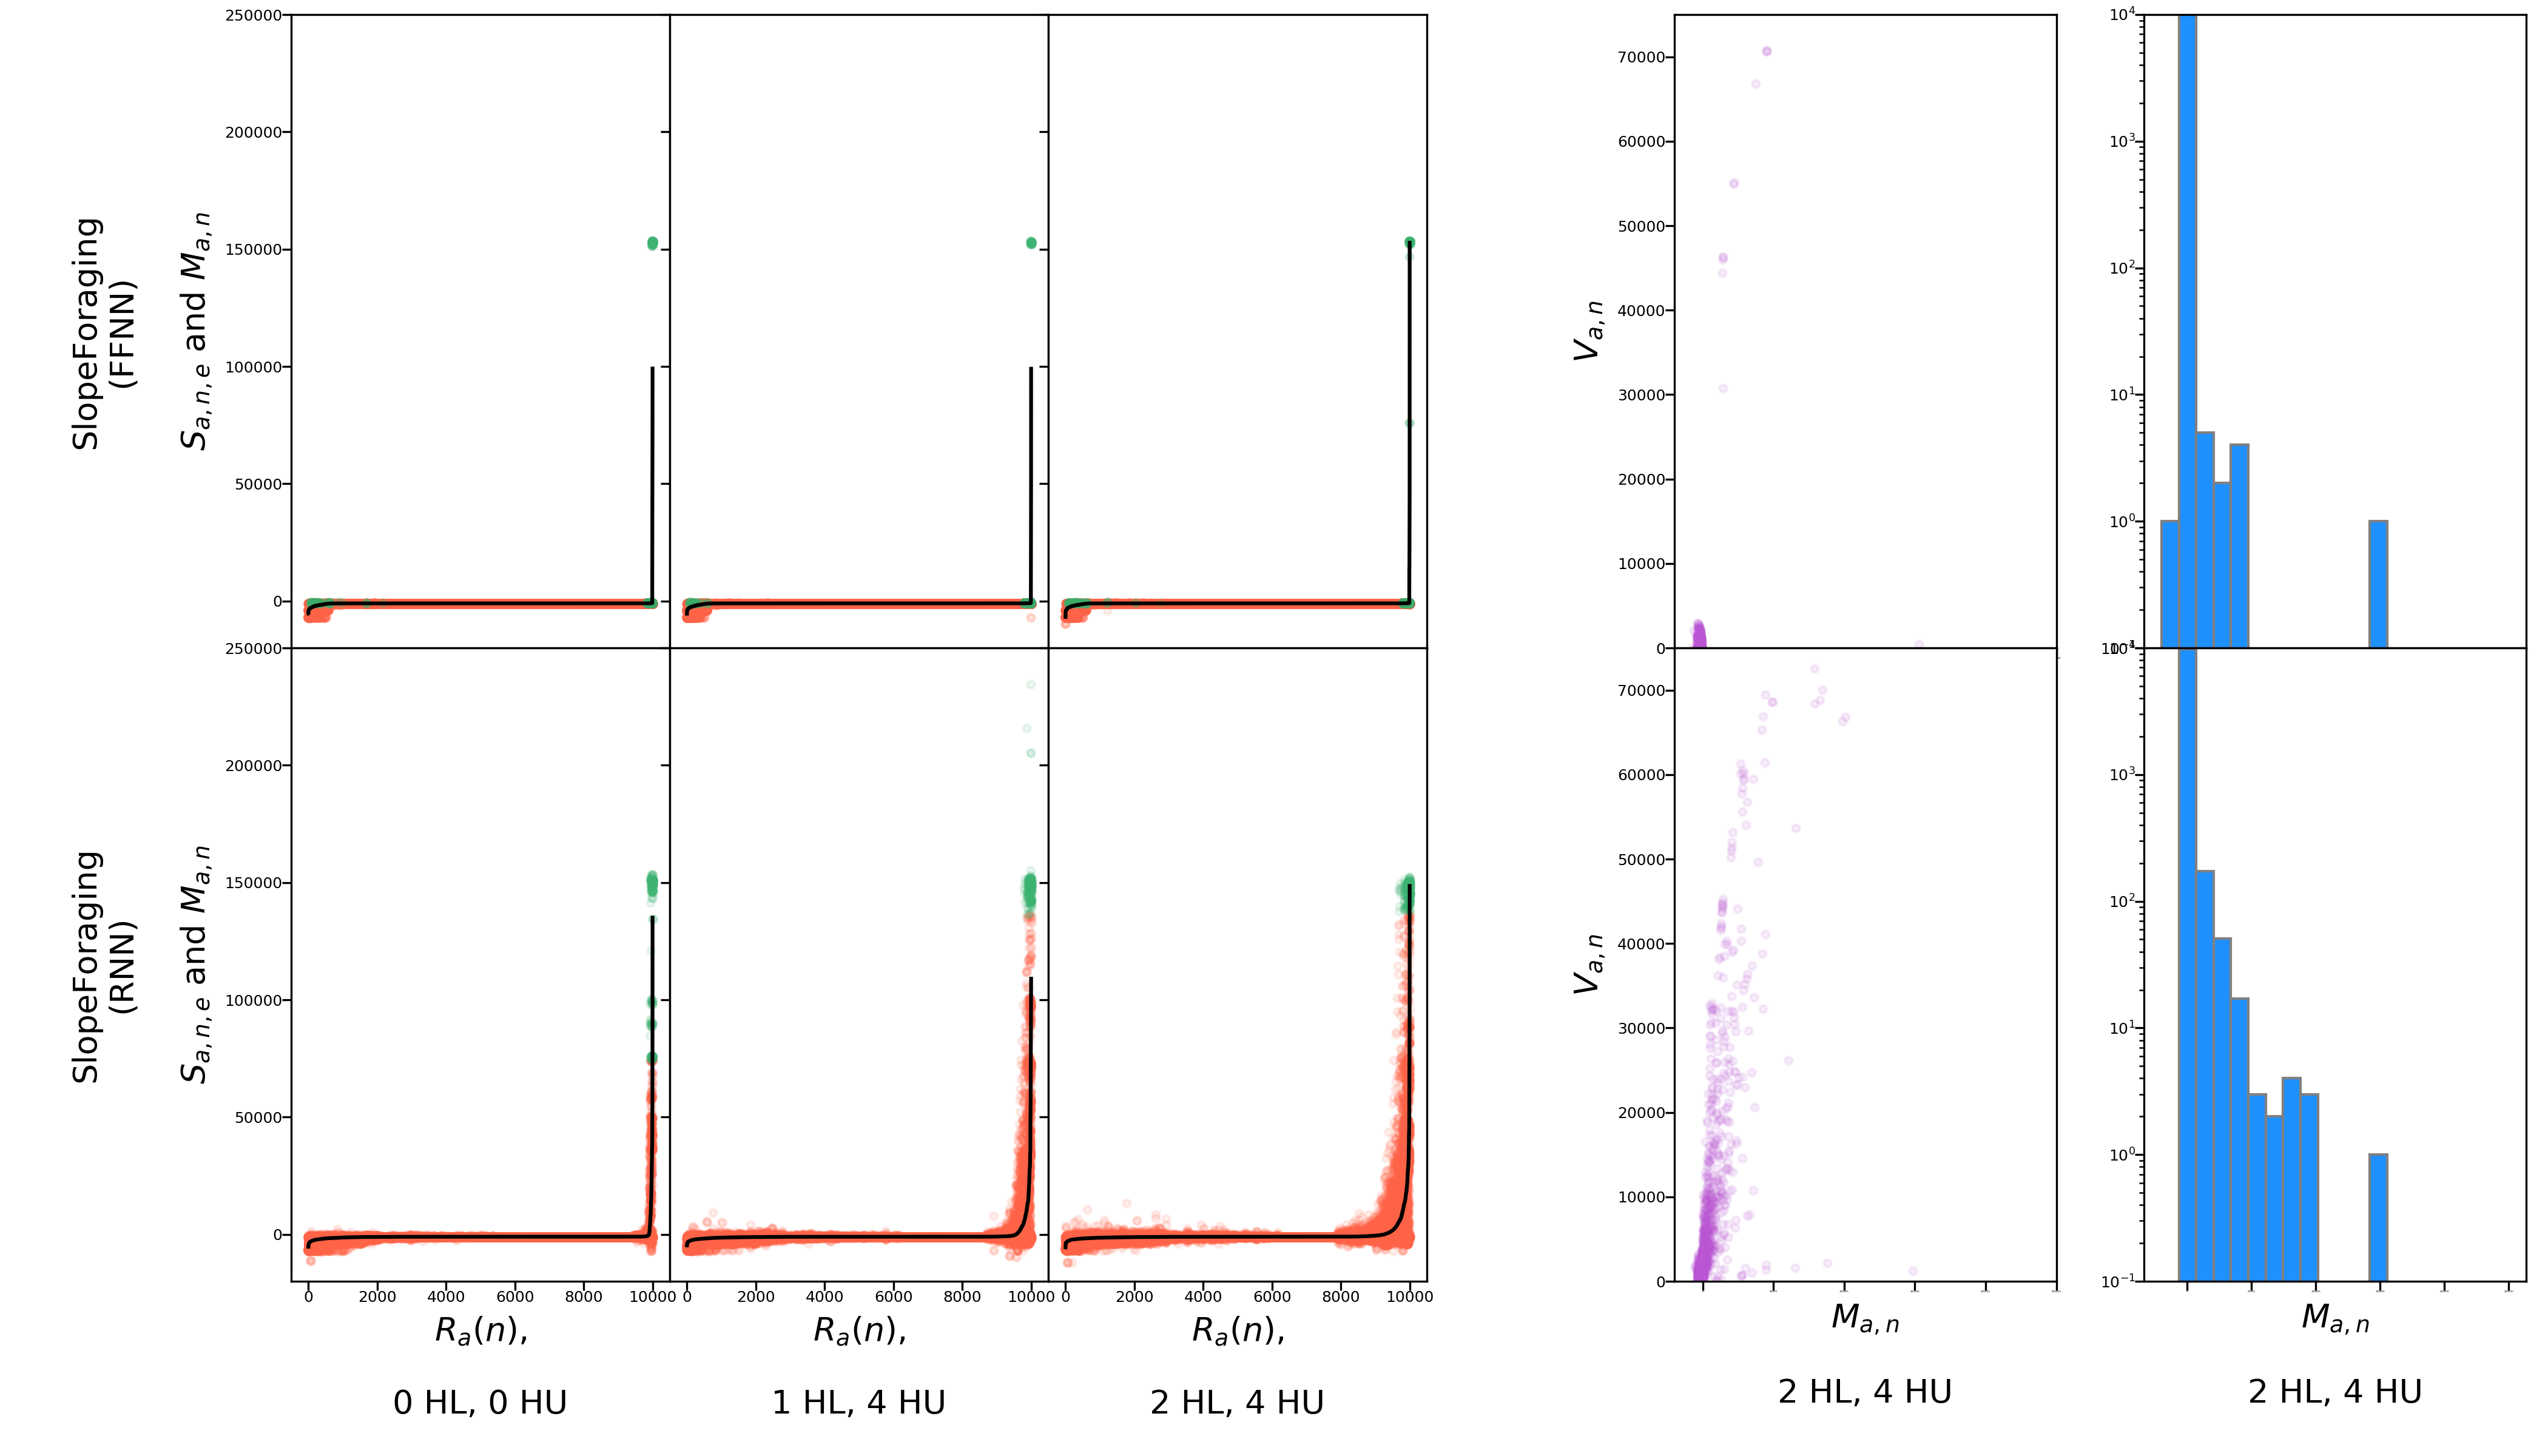
\includegraphics[width=1.0\textwidth]{incremental_rewards.png}
\caption{RWG Analysis with incremental rewards}
\label{fig:incremental}
\end{figure}

Looking at the 6 mean plots in Figure \ref{fig:incremental} compared to Figure \ref{fig:sparse}, we see that with incremental rewards, the solutions do in fact form more of a gradient towards the right end of the plot, in particular for RNNs (bottom row). 
This means that a lot of the solutions in the landscape are partially successful at retrieving resources. 
However, the landscape is still largely flat. 
This is presumably because most solutions in the landscape don't even get to the point of picking up a resource from the source.\\ 

Thus the answer to Hypothesis 1.1 is:\\

\textbf{Answer 1.1:} Rewarding agents for partial retrieval of the resource creates a smoother fitness gradient, but the landscape is still largely flat.\\

In order to further smooth the fitness landscape there would need to be rewards for partial progress up the slope, but the problem with this is that it is likely to disincentivise the collector behaviour in evolution.
Why would an agent stay at the nest and collect resource when they are rewarded for going up the slope? 
Additionally, while this problem is simple enough to smooth the fitness gradient in this way, such smoothing may not be possible for other more complex problems.
The purpose of this research is to understand how to use AI to find good solutions with minimal (if any) human intervention.\\

Moreover, the flatness of the landscape is, to some extent, inherent to this task.
This is a problem common in evolutionary computation known as the bootstrapping problem \cite{Silva:EC:2016, Wei:ALR:2019}.
Bootstrapping is "when the task is too demanding for the fitness function to apply any meaningful selection pressure on a randomly generated population of initial candidate solutions" \cite{Silva:EC:2016}.
The bootstrapping problem often occurs when the goal behaviour is complex relative to the very simple available actions \cite{Wei:ALR:2019}.
For this problem, the available actions are primitives like 'move forward one tile' and 'move backward one tile'.
When putting together sequences of these actions, most sequences will obviously not be very successful.
There are many proposed solutions to solving the bootstrapping problem and they fall under the broad categories of inserting human knowledge into the learning process or increasing the diversity of solutions \cite{Silva:EC:2016}.
Smoothing the landscape falls under the former category, but this family of techniques has some shortcomings, in particular it reduces the potential for automation and risks the experimenter introducing negative biases.
Using rwg to find a seed falls under the second category; it has the shortcoming of additional computation, which may not scale well for problems with larger solution spaces, but for those problems there is a wealth of alternative techniques for increasing diversity, such as novelty search.
In keeping with the spirit of AI, I have chosen to continue using the more challenging fitness function.

\end{document}